
%
%
% Module: carrier_recovery_matlab_exercise
%
% Author: Michael Kramer
%
%

Simulate the PLL system shown in Figure \ref{fig: PLL} using
\matlab.  As with the DLL simulation, you will have to simulate
the PLL on a sample by sample basis. 

Use equation (\ref{eq: phase_update}) to implement your NCO in 
\matlab. However to ensure that the phase term does not grow
to infinity you should use addition modulo $2 \pi$ in the phase update
relation.  This can be done by checking to see if $\theta(n) > 2 \pi$,
and if so, replace it with $\theta(n) = \theta(n) - 2 \pi$.

Figure \ref{fig: pll_output} illustrates how the proposed PLL will
behave when given a modulated BPSK waveform.  In this case
the transmitted carrier frequency was set to $\tilde{\lambda}_c =
\frac{\pi}{2} + \frac{\pi}{1024}$ to simulate a frequency offset.

\begin{figure}[ht]
   \begin{center}
      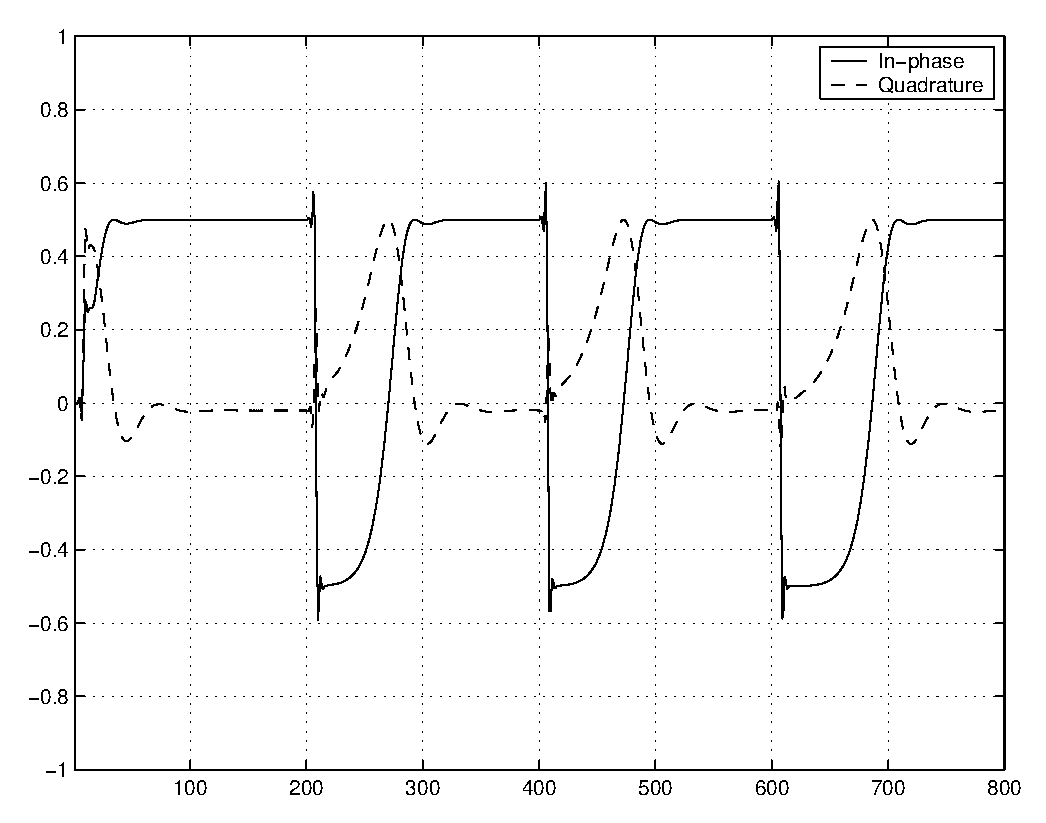
\epsfig{file=pll_output.eps,width=10cm}
      \caption{Output of PLL sub-system for BPSK modulated carrier.}
      \label{fig: pll_output}
   \end{center}
\end{figure}

Note that each time an amplitude transition occurs in the BPSK
waveform, this is equivalent to a phase shift of the carrier
by $\frac{\pi}{2}$.  Immediately after this phase change occurs
the PLL begins to adjust the phase to force the quadrature
component to zero (and the in-phase component to $\frac{1}{2}$).
Why would this phase detector not work in a real BPSK environment?
